%competidores
\section{Tecnologías competidoras}

\subsection{Radio Frequency Identification - RFID}
RFID o identificación por radiofrecuencia en español, un término que describe a un dispositivo electrónico que utiliza radiofrecuencia o variaciones de campo magnético para comunicarse; que es puesto a un artículo. Los dos componentes de un sistema RFID son la etiqueta, que es el dispositivo que identifica al artículo que queremos ubicar, y el lector, que reconoce la presencia de las etiquetas,  con el fin de leer la información almacenada en ellas.
El lector obtiene la información de los elementos presentes etiquetados e informa a otro sistema de ello, siendo esta un software que se interpone entre los lectores y las aplicaciones;  middleware RFID. \cite{2006_BillGlover_BOOK}
\begin{figure} 	
	\centering
	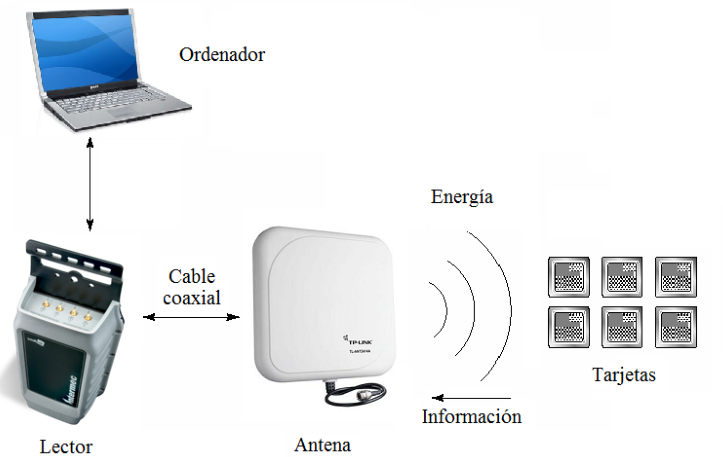
\includegraphics[width=0.7\linewidth]{funcarfid.png}
	\caption{Tecnología RFID.}
	\label{fig:rfid}
\end{figure}
\\
RFID se está convirtiendo en una tecnología rentable, capaz de recibir y transmitir varios metros la información.\cite{2011_Coskun_BOOK} El sistema se compone de tres componentes básicos: una etiqueta en el artículo, un lector y una computadora host, vea la figura (\ref{fig:rfid}).  Las etiquetas son pequeños chips semiconductores y con antenas miniaturizadas dentro de algún tipo de empaque. Se puede rastrear e identificar a objetos o personas de forma inalámbrica por el par lector / host. \cite{2006_BillGlover_BOOK}
Por lo general, la etiqueta lee su memoria interna de datos y lo intercambia con la antena (lector), de forma codificada transmitiendo los datos.\cite{2005_Landt}
\\
El RFID aumenta la productividad y la comodidad. Utilizado para comunicar información digital entre diferentes espacios físicos y un objeto en móvil o entre objetos en movimiento. Para transferir de la etiqueta al lector utiliza el principio de retrodispersión modulada -fenomeno físico donde las ondas inciden en un material y luego son reflejadas en el mismo ángulo, volviendo a la fuente que las produjo -. \cite{2005_Landt}
\\
Esta tecnología ofrece beneficios para la gestión de la cadena de suministro, el control de inventario y suministro, gestión de la seguridad (identificación, ubicación, seguimiento y supervisión de personas y/o objetos), transporte y distribución: camiones, almacenes, etiquetas de peaje de carreteras y gestión de flotas, seguimiento de contenedores, entre otras.\cite{2007_Hunt_BOOK,2005_Weinstein}

\begin{figure} 	
	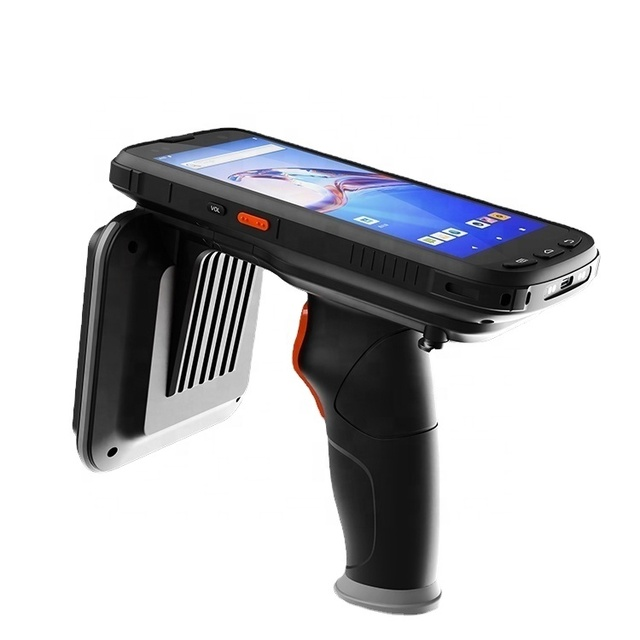
\includegraphics[width=0.5\linewidth]{lectorRFID.jpg}
	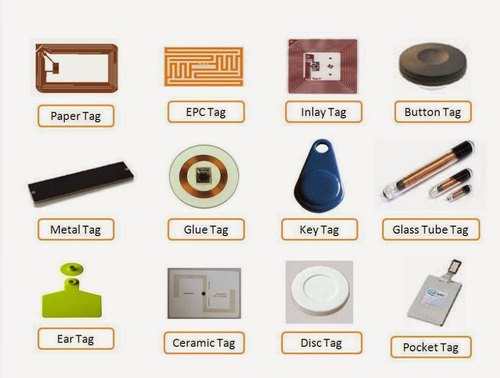
\includegraphics[width=0.5\linewidth]{tagRFID.jpg}
	\caption{Lector RFID y tipos de etiquetas.}
	\label{fig:rfid2}
\end{figure}

\textbf{Ventajas}: Alineación no es necesaria; un escaneo no requiere línea de visión, dado que es posible escanear varios artículos al mismo tiempo. Variedad de factores de forma; las etiquetas varían en tamaño. Seguimiento a nivel de artículo; identificación de forma única entre millones. Además, es posible la reescritura en algunas etiquetas, como también de una sola escritura. Transmisión de datos de corto y largo alcance. No requiere alimentación eléctrica interna las etiquetas pasivas, pero si las activas.\cite{2006_BillGlover_BOOK,2011_Coskun_BOOK}
\\
\textbf{Desventajas}: Solo para ubicar objetos y personas, no útil para pagos. Es necesario la compra del lector y el software.\cite{2005_Landt} Precio de las etiquetas dependendiendo del rango de lectura, baterías para las etiquetas activas.

\subsection{Near-Field Communication - NFC}
NFC o Comunicación de campo cercano en español, es una tecnología de comunicación inalámbrica entre dos dispositivos equipados con NFC, con una alta frecuencia de 13,56 Mhz utilizada originalmente por RFID, bajo ancho de banda y de corto alcance. La mayoría de los teléfonos móviles tienen incorporados esta tecnología, permitiendo la comunicación entre un teléfono móvil en un extremo y/o un lector NFC o una etiqueta NFC en el otro extremo.
La tecnología NFC permite el pago electrónico, emisión de billetes electrónicos, sevicios de fidelización, identificación, control de acceso, distribución de contenido, publicidad inteligente, transferencia de datos/dinero y otros servicios. \cite{2011_Coskun_BOOK}
\begin{figure} 	
	\centering
	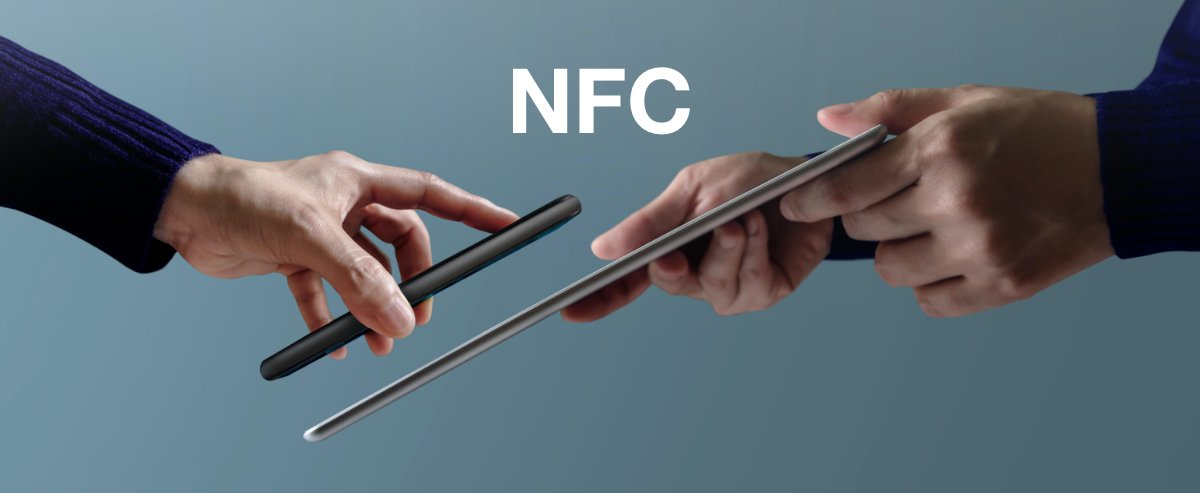
\includegraphics[width=0.4\linewidth]{nfc1.jpg}
	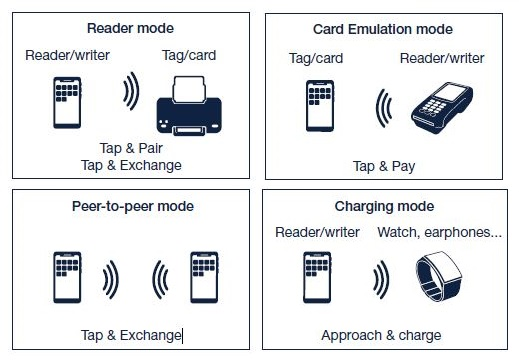
\includegraphics[width=0.7\linewidth]{nfc-mode-operations.jpg}
	\caption{Tecnología NFC entre dos telefónos móviles y sus modos de operación.}
	\label{fig:nfc}
\end{figure}
\\
La comunicación de campo cercano implica dos chips NFC, cuando uno de los dispositivos se coloca cerca del chip o telefóno móvil puede solicitar al dispositivo realizar una acción específica. Por ejemplo, abrir una página web, marcar un número telefóno, compartir imagen o video, entre otros.\cite{2012_Waters_BOOK}
\\
La tecnología necesita siempre dos dispositivos, un iniciador; que genera activamente una señal de RF controlando el intercambio de datos donde la solicitud es respondida por un objetivo pásivo (móvil). Existen dos modos de comunicación: activo y pasivo. Activos donde ambos dispositivos generan sus propios campos eléctricos, lo hacen semidúplex; desactivando su campo de RF hasta que ningún otro dispositivo transmita. Ambos dispositivos suelen tener fuentes de alimentación. En cambio, el modo pasivo; solo uno genera el campo, donde el dispositivo de destino responde a esa llamada, estando en escucha y luego procesa la transferencia de datos.\cite{2012_Curran}
\\
\textbf{Ventajas}: Simple de usar; sin escaneo o sostener su teléfono, ni siquiera golpear físicamente los dispositivos, intercambio de datos seguro inherente debido a la comunicación de corto alcance, Emparejamiento implícito de parejas de parejas expresando su voluntad al realizar la comunicación. Modos de funcionamiento: reader/writer, peer-to-peer, and card emulation.\cite{2011_Coskun_BOOK}
\\
\textbf{Desventajas}: Comunicación de corto alcance, limitado a una distancia entre los dos dispositivos de hasta 10 cm.\cite{2012_Curran} Comparando con el QR es necesario comprar etiquetas de un costo no tan elevado y es necesario que el móvil tenga incorporado la tecnología.\cite{2011_Coskun_BOOK} Consumo prolongado de la batería del móvil.\cite{2012_Waters_BOOK} 

\subsection{Bluetooth Beacons}
BLE beacons o balizas BLE en español, son balizas con pequeños transmisores de radio, que se comunican a través de Bluetooth Low Energy. Las balizas son colocados en ubicaciones de forma estratégicamente para que se transmitan las señales de Bluetooth de baja energía en un rango determinado (depende del hardware).  A través de canales de BLE, se envían un número de identificación, 10 veces por segundo, donde un dispositivo con bluetooth en las cercanias de la baliza los recoge, este número es capaz de desencadenar una acción específica relevante para la ubicación (descargar una aplicación o contenido). \cite{Adarsh2021} 
\begin{figure} 	
	%\centering
	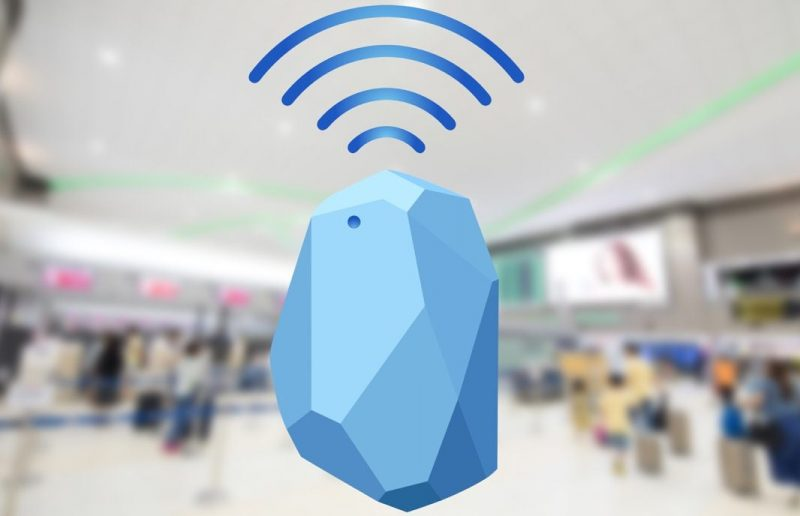
\includegraphics[width=0.4\linewidth]{beacon1.jpg}
	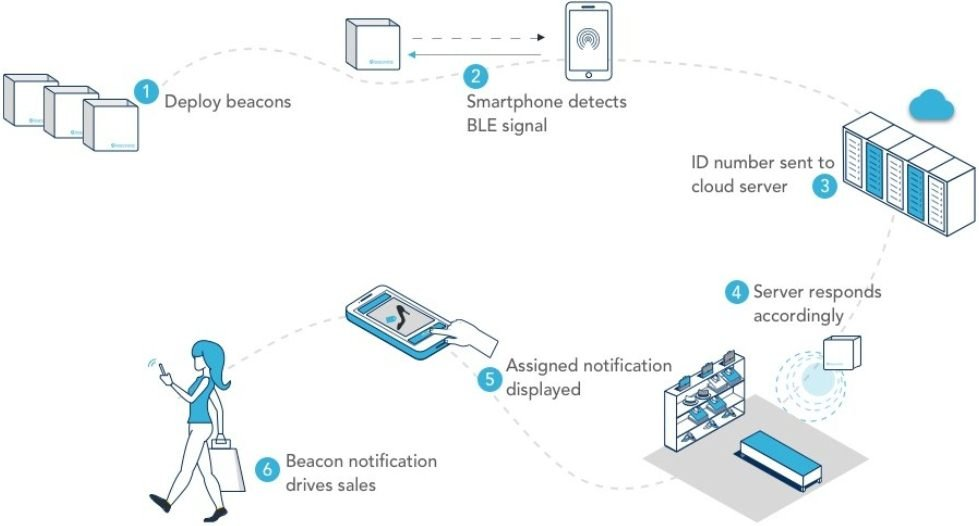
\includegraphics[width=0.6\linewidth]{beacon2.jpg}
	\caption{Tecnología Beacons BLE.}
	\label{fig:beacons}
\end{figure}

Esta tecnología tiene aplicaciones en el manejo de problemas de colocación o gestión de inventario, dado que el posicionamiento de los artículos es cambiante entre entregas. \cite{Octaviani2020} También son usados como marketing por proximidad, registro hiperlocal; ubicar a los visitantes con precisión, anuncios de reorientación, seguimiento de activos; las etiquetas pueden estar compuestas con sensores (luz, sonido, temperatura) que permiten el seguimiento de otros objetos y por último, navegación en interiores; marca los lugares importantes e indica la ruta recomendada. \cite{Adarsh2021}
\\
\textbf{Ventajas}: Transmisión de datos a 80 metros y también permite que el dispositivo móvil determine su ubicación siendo anónimo.\cite{Adarsh2021,Chawathe2008} 
\\
\textbf{Desventajas}: La propagación de la señal en entornos interiores es compleja y se ve afectada por muchos factores, interferencia de otros dispositivos, entre otros. El área de ubicación tiene un modelo simple como un elipsoide.\cite{Chawathe2008} El costo de la batería y de la tecnología Beacon BLE.

\subsection{Augmented reality (AR)}
La realidad aumentada superpone el mundo real con contenido digital, a través de un dispositivo tecnológico con información virtual generada por este. Es una vista en vivo, de forma directa o indirecta, del espacio físico real cuyos elementos son aumentados por algún medio audiovisual que son generados por el dispositivo. Por ejemplo, pueden permitir ver el interior de un edificio desde la acera, usando sus teléfono móviles. Alineando la pantalla del teléfono con el edificio, viendo como el mundo real es superpuesto por imagenes, videos, sonido, entre otros.\cite{2011BOOK,2012_Waters_BOOK}
%arItems
\begin{figure} 	
	\centering
	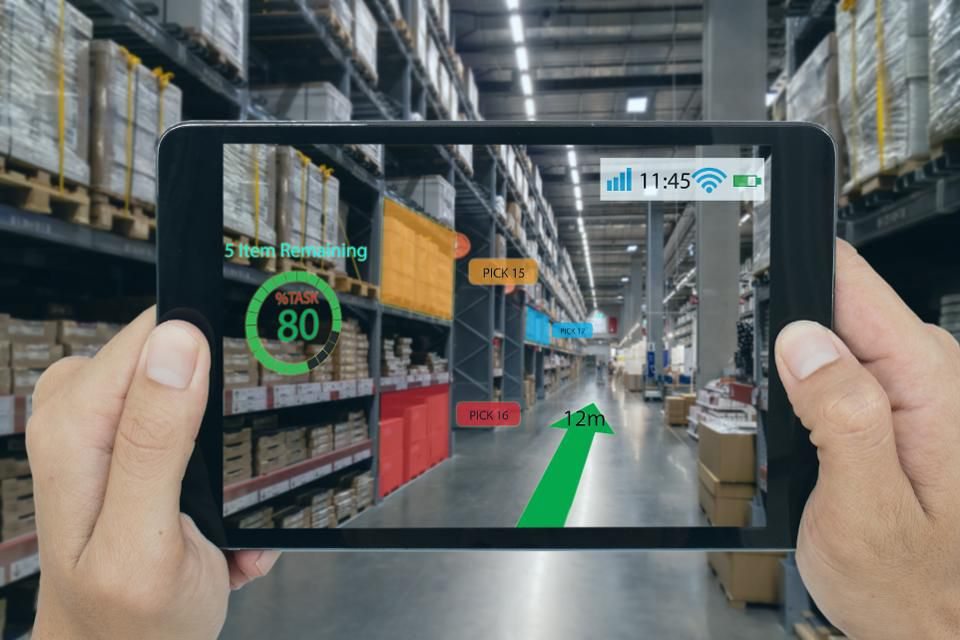
\includegraphics[width=0.5\linewidth]{arItems.jpg}
	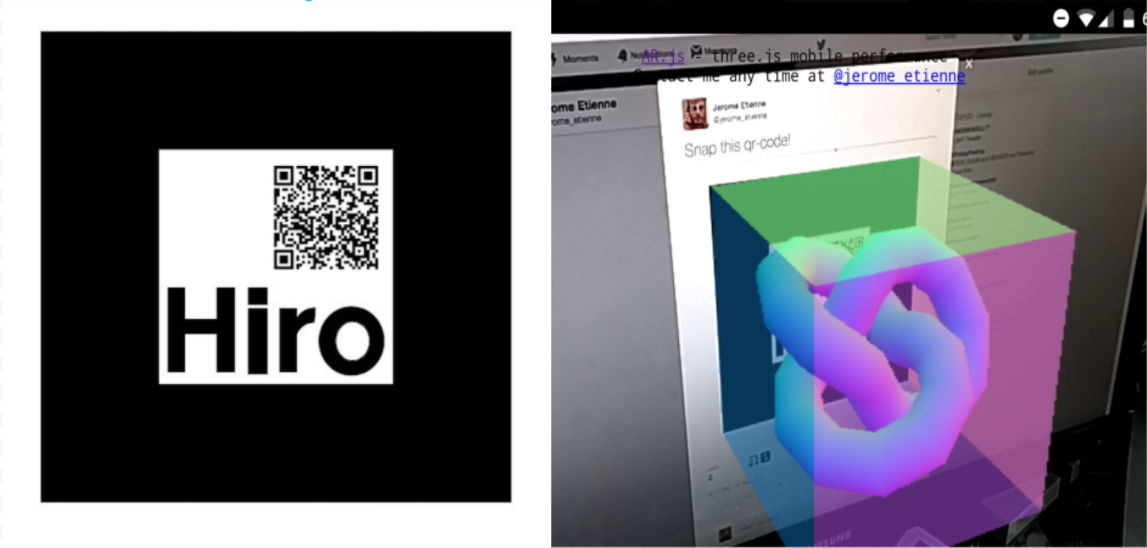
\includegraphics[width=0.5\linewidth]{arconqr.png}
	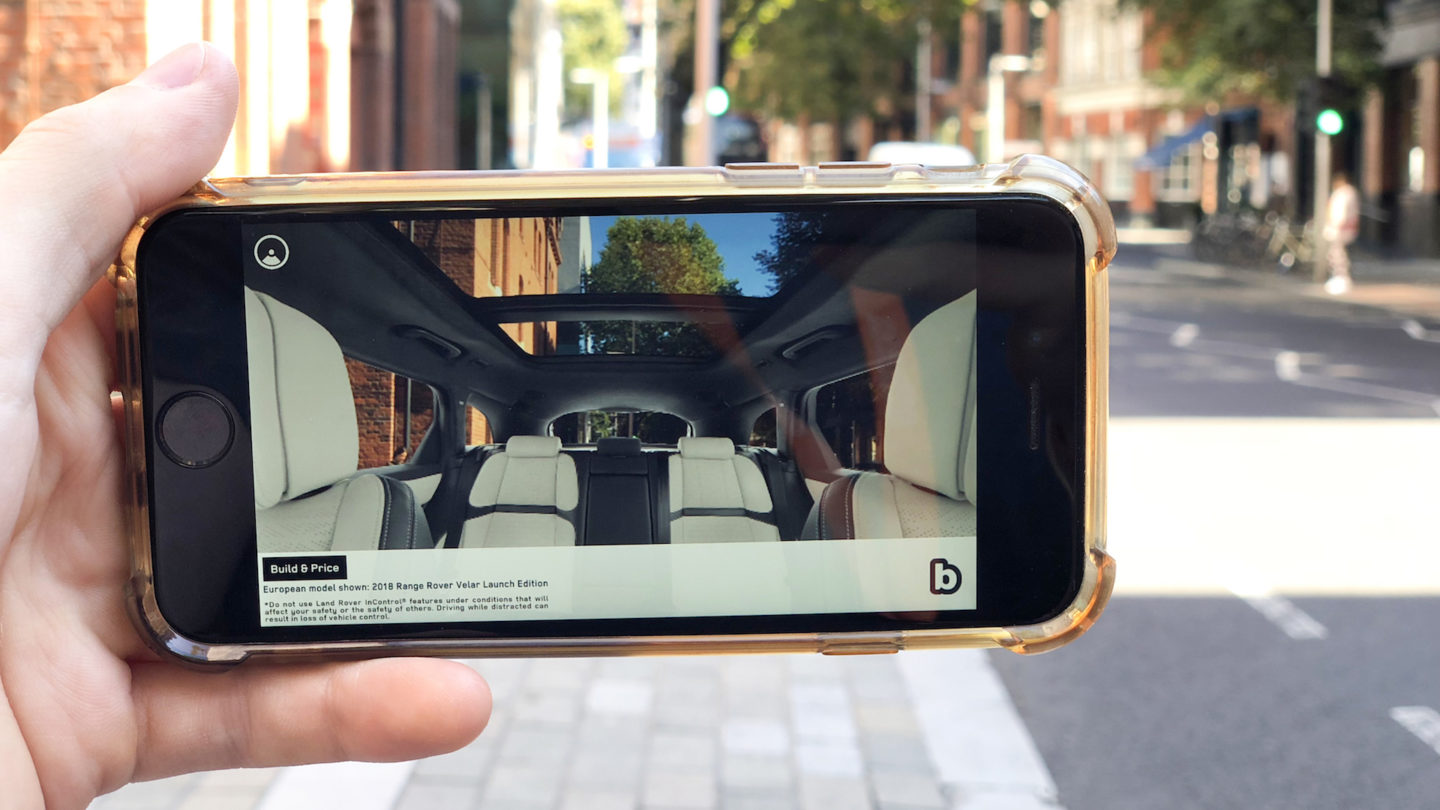
\includegraphics[width=0.5\linewidth]{Augmented-reality-examples-_-Auto-_-Jaguar-Land-Rover-_-Blippar-carousel.jpg}
	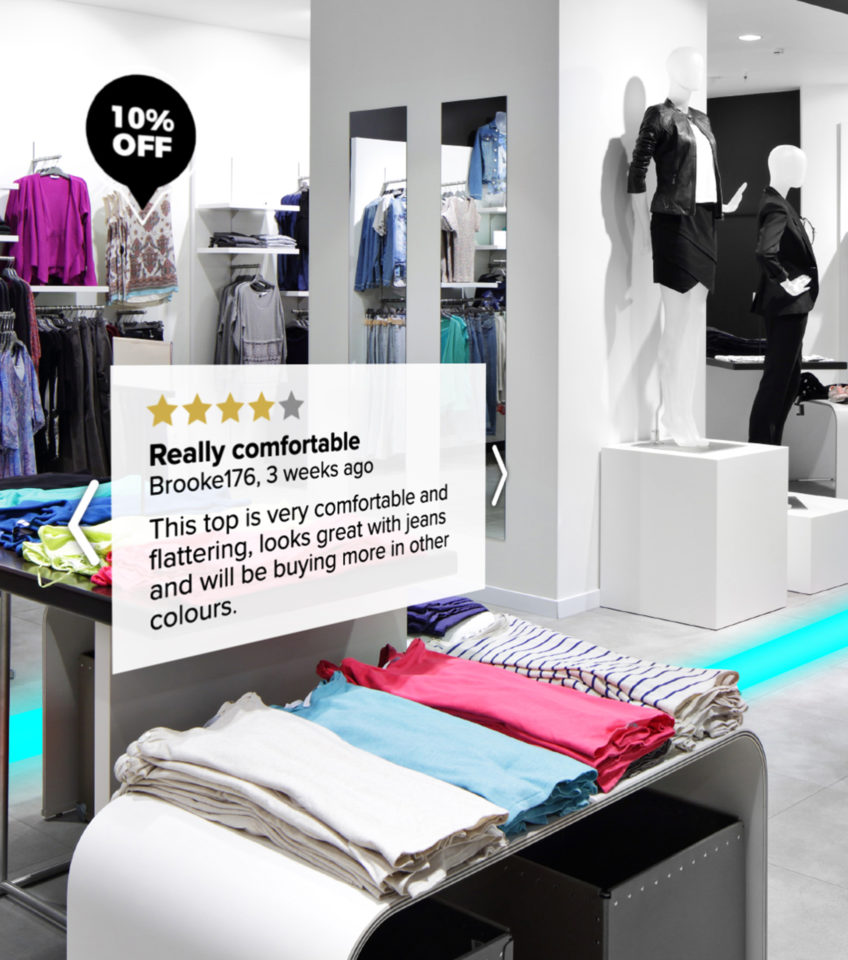
\includegraphics[width=0.3\linewidth]{Augmented-reality-in-retail-_-Blippar.jpg}
	\caption{Tecnología de Realidad Aumentada.}
	\label{fig:ar}
\end{figure}
La tecnología tiene aplicaciones como Fig.(\ref{fig:ar}),  un sistema de navegación de interior interactivo, y el uso de la tecnología de realidad aumentada para superporner señales de dirección.También en el área de salud; estudio del corazón humano, anatomía del cuerpo humano, entre otros.	En el comercio, ayuda a mejorar la experiencia de los clientes, mostrando detalles o información del artículo (precio, nombre, modo de uso, entre otros). \cite{2021_Ong_THESIS,2021_Romli,2021_Fernandes} 
\\
\textbf{Ventajas}: el usuario puede experimentar el objeto virtual con más detalle desde varios ángulos, con lo cuál facilita mayor información y agiliza las tareas. \cite{2021_Romli}
\\
\textbf{Desventajas}: es necesario que el software sea compatible con la tecnologia AR, precio del software de realidad aumentada, dificultad de interacción con el usuario (Interfaz gráfica), requiere más tiempo de uso, problemas técnicos dados por el teléfono móvil.\cite{2018_Gavilanes}

\subsection{Image Recognition}

El reconocimiento de imágenes, es un conjunto de técnicas para identificar y analizar imágenes permitiendo la automatización de una tarea específica. Es capaz de reconocer lugares, objetos, personas y otro tipos de elementos que estan dentro de una imagen, sacando conclusiones para la toma de decisiones. Es una subcategoría de visión por computadora e inteligencia artificial, basado principalmente en Deep Learning, subcategoría de Machine Learning (uso de una red neuronal artificial entrenada mediante un conjunto de datos anotados).\cite{deepomatic.com2021,Wu2015}

\begin{figure} 	
	%\centering
	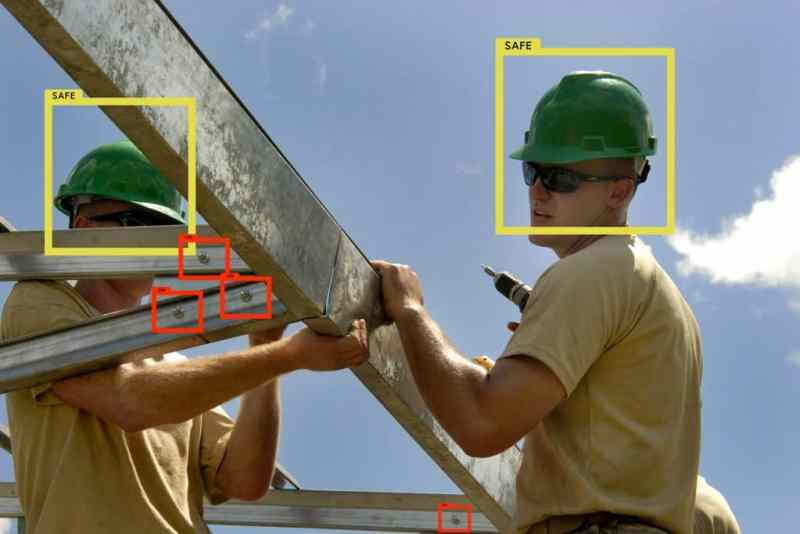
\includegraphics[width=0.5\linewidth]{imagerecognition.jpg}
	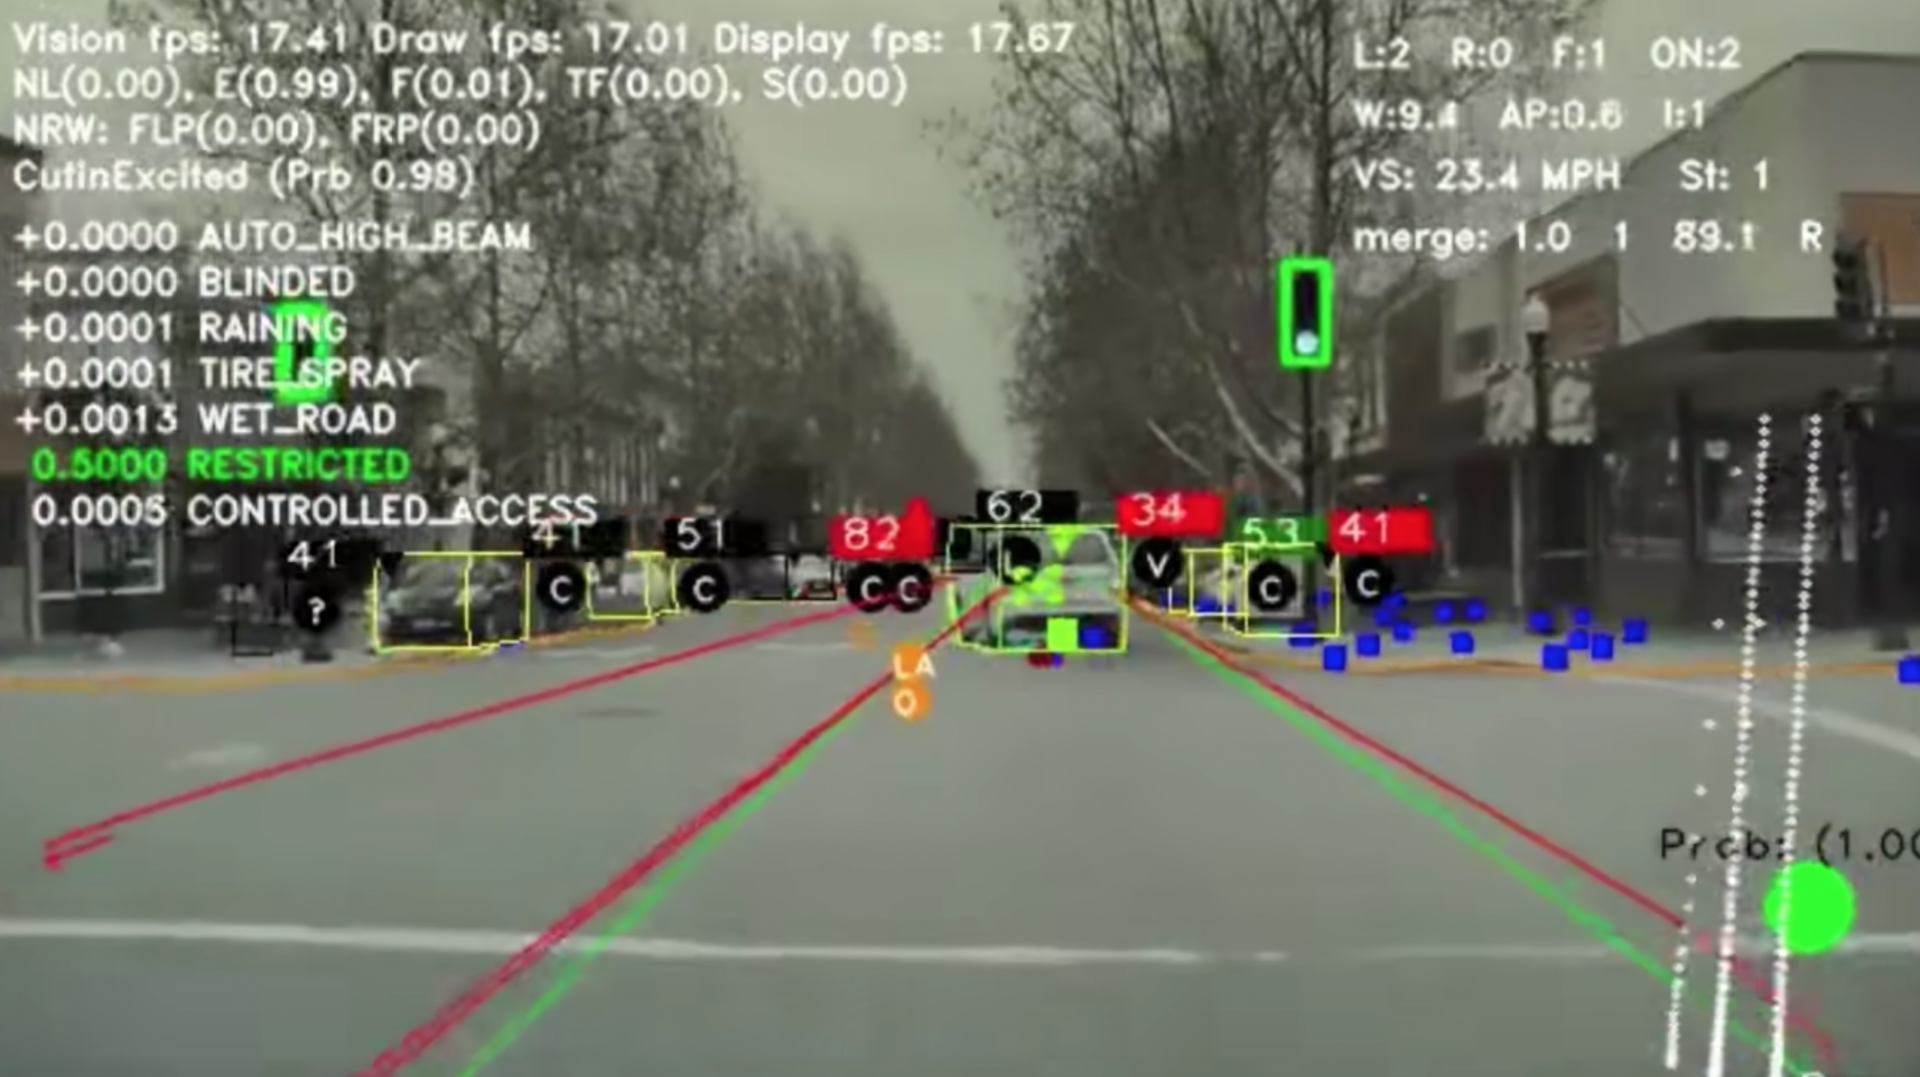
\includegraphics[width=0.5\linewidth]{teslaautopilot.png}
	\caption{Tecnología de Reconocimiento de imagen.}
	\label{fig:Irecog}
\end{figure}

Por ejemplo, el etiquetado de una imagen, ubicar algún objeto principal de una imagen o el guiado de un automóvil autónomo.
Dentro de ella tenemos, clasficación de imágenes; identificar la categoría a la que pertenece una imagen, detección de objetos; ubicar el elemento en la imagen -con un cuadro delimitador- Fig.(\ref{fig:Irecog}) , segmentación; detección de un elemento con precisión de pixel para automóviles autónomos, etiquetado; asignación de una o más etiquetas a una imagen en particular.  \cite{deepomatic.com2021}
\\
\textbf{Ventajas}: Puede reconocer cualquier elemento dentro de la imagen, incluso códigos QR u otros tipos. Solo es necesario la aplicación, una foto con su cámara o cualquier imagen y con la conexión a Internet, se obtiene resultados o contenido relacionado. \cite{lens.google2021}
\\
\textbf{Desventajas}: El reconocimiento de imagen debe estar entrenada (Hardware y Software). \cite{deepomatic.com2021,Wu2015} 

\subsubsection{Bixby Vision}
Bixby Vision es un asistente virtual disponible en teléfonos móviles samsungs, las funciones disponibles son: traducción de texto de un idioma a otra en la vista previa en vivo de la pantalla, permite realizar búsquedas de imagenes similares a la imagen tomada con la cámara, con ello podemos realizar una búsqueda de artículos similares. Lectura de un código QR, descriptor de escena, identificador de objetos, lector de texto desde una imagen, entre otros. \cite{samsung.com2021}
\begin{figure} 	
	%\centering
	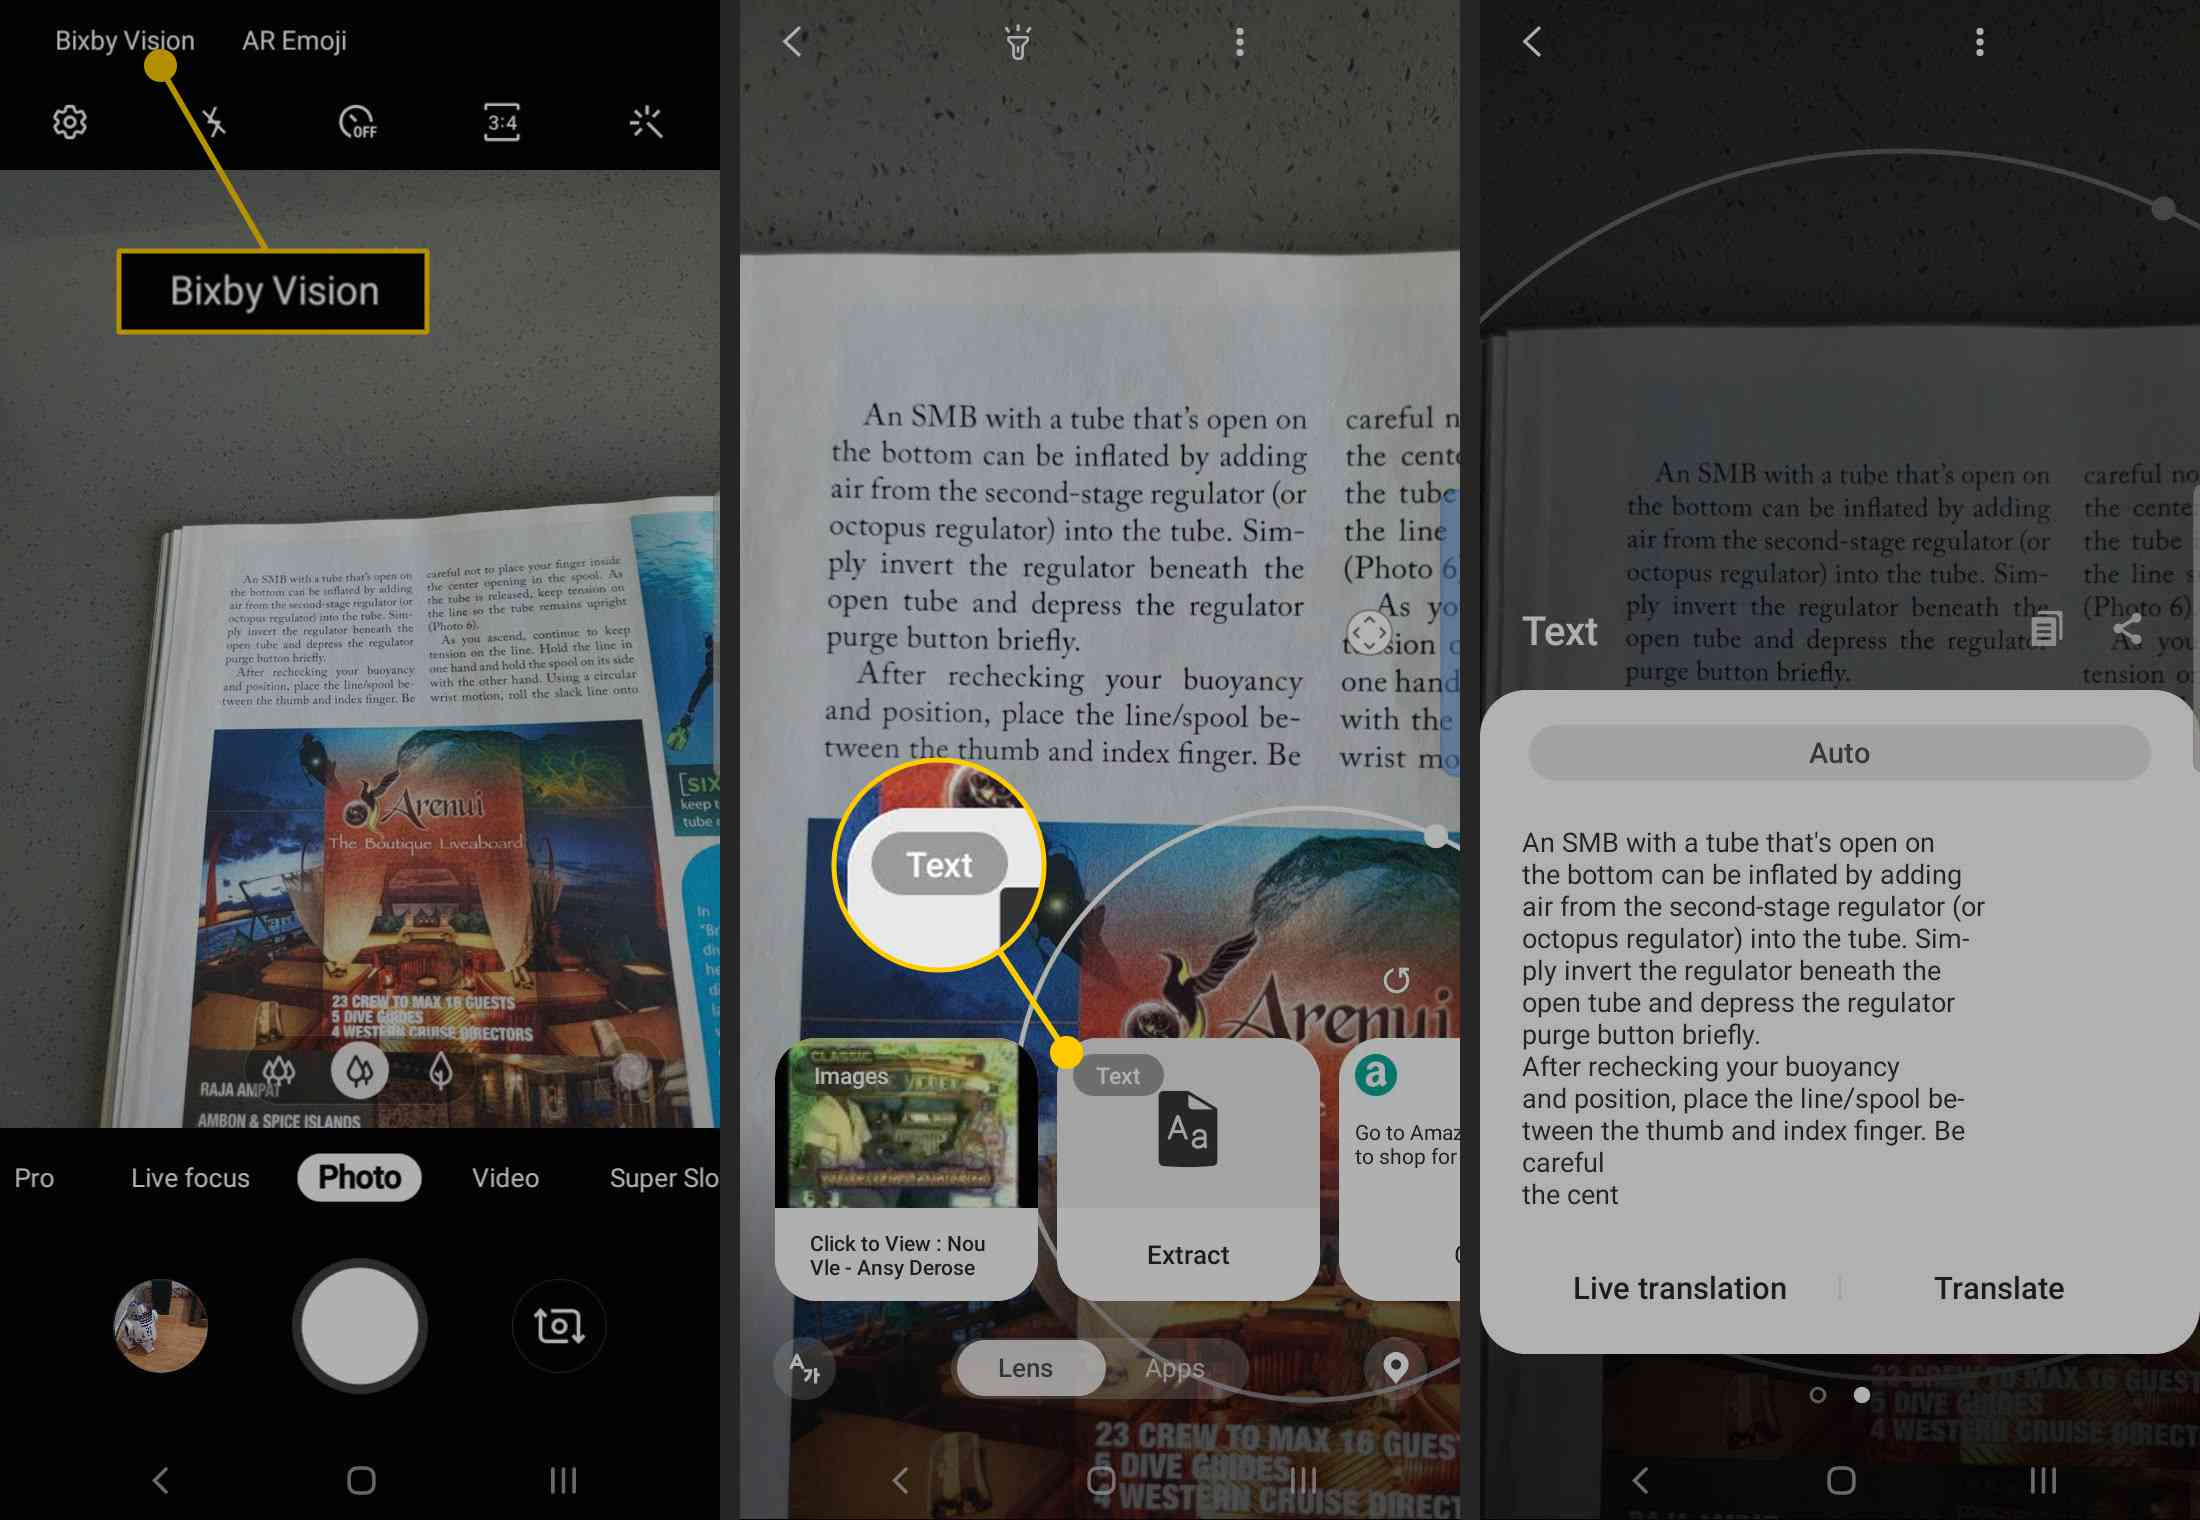
\includegraphics[width=0.5\linewidth]{bixby1.jpg}
	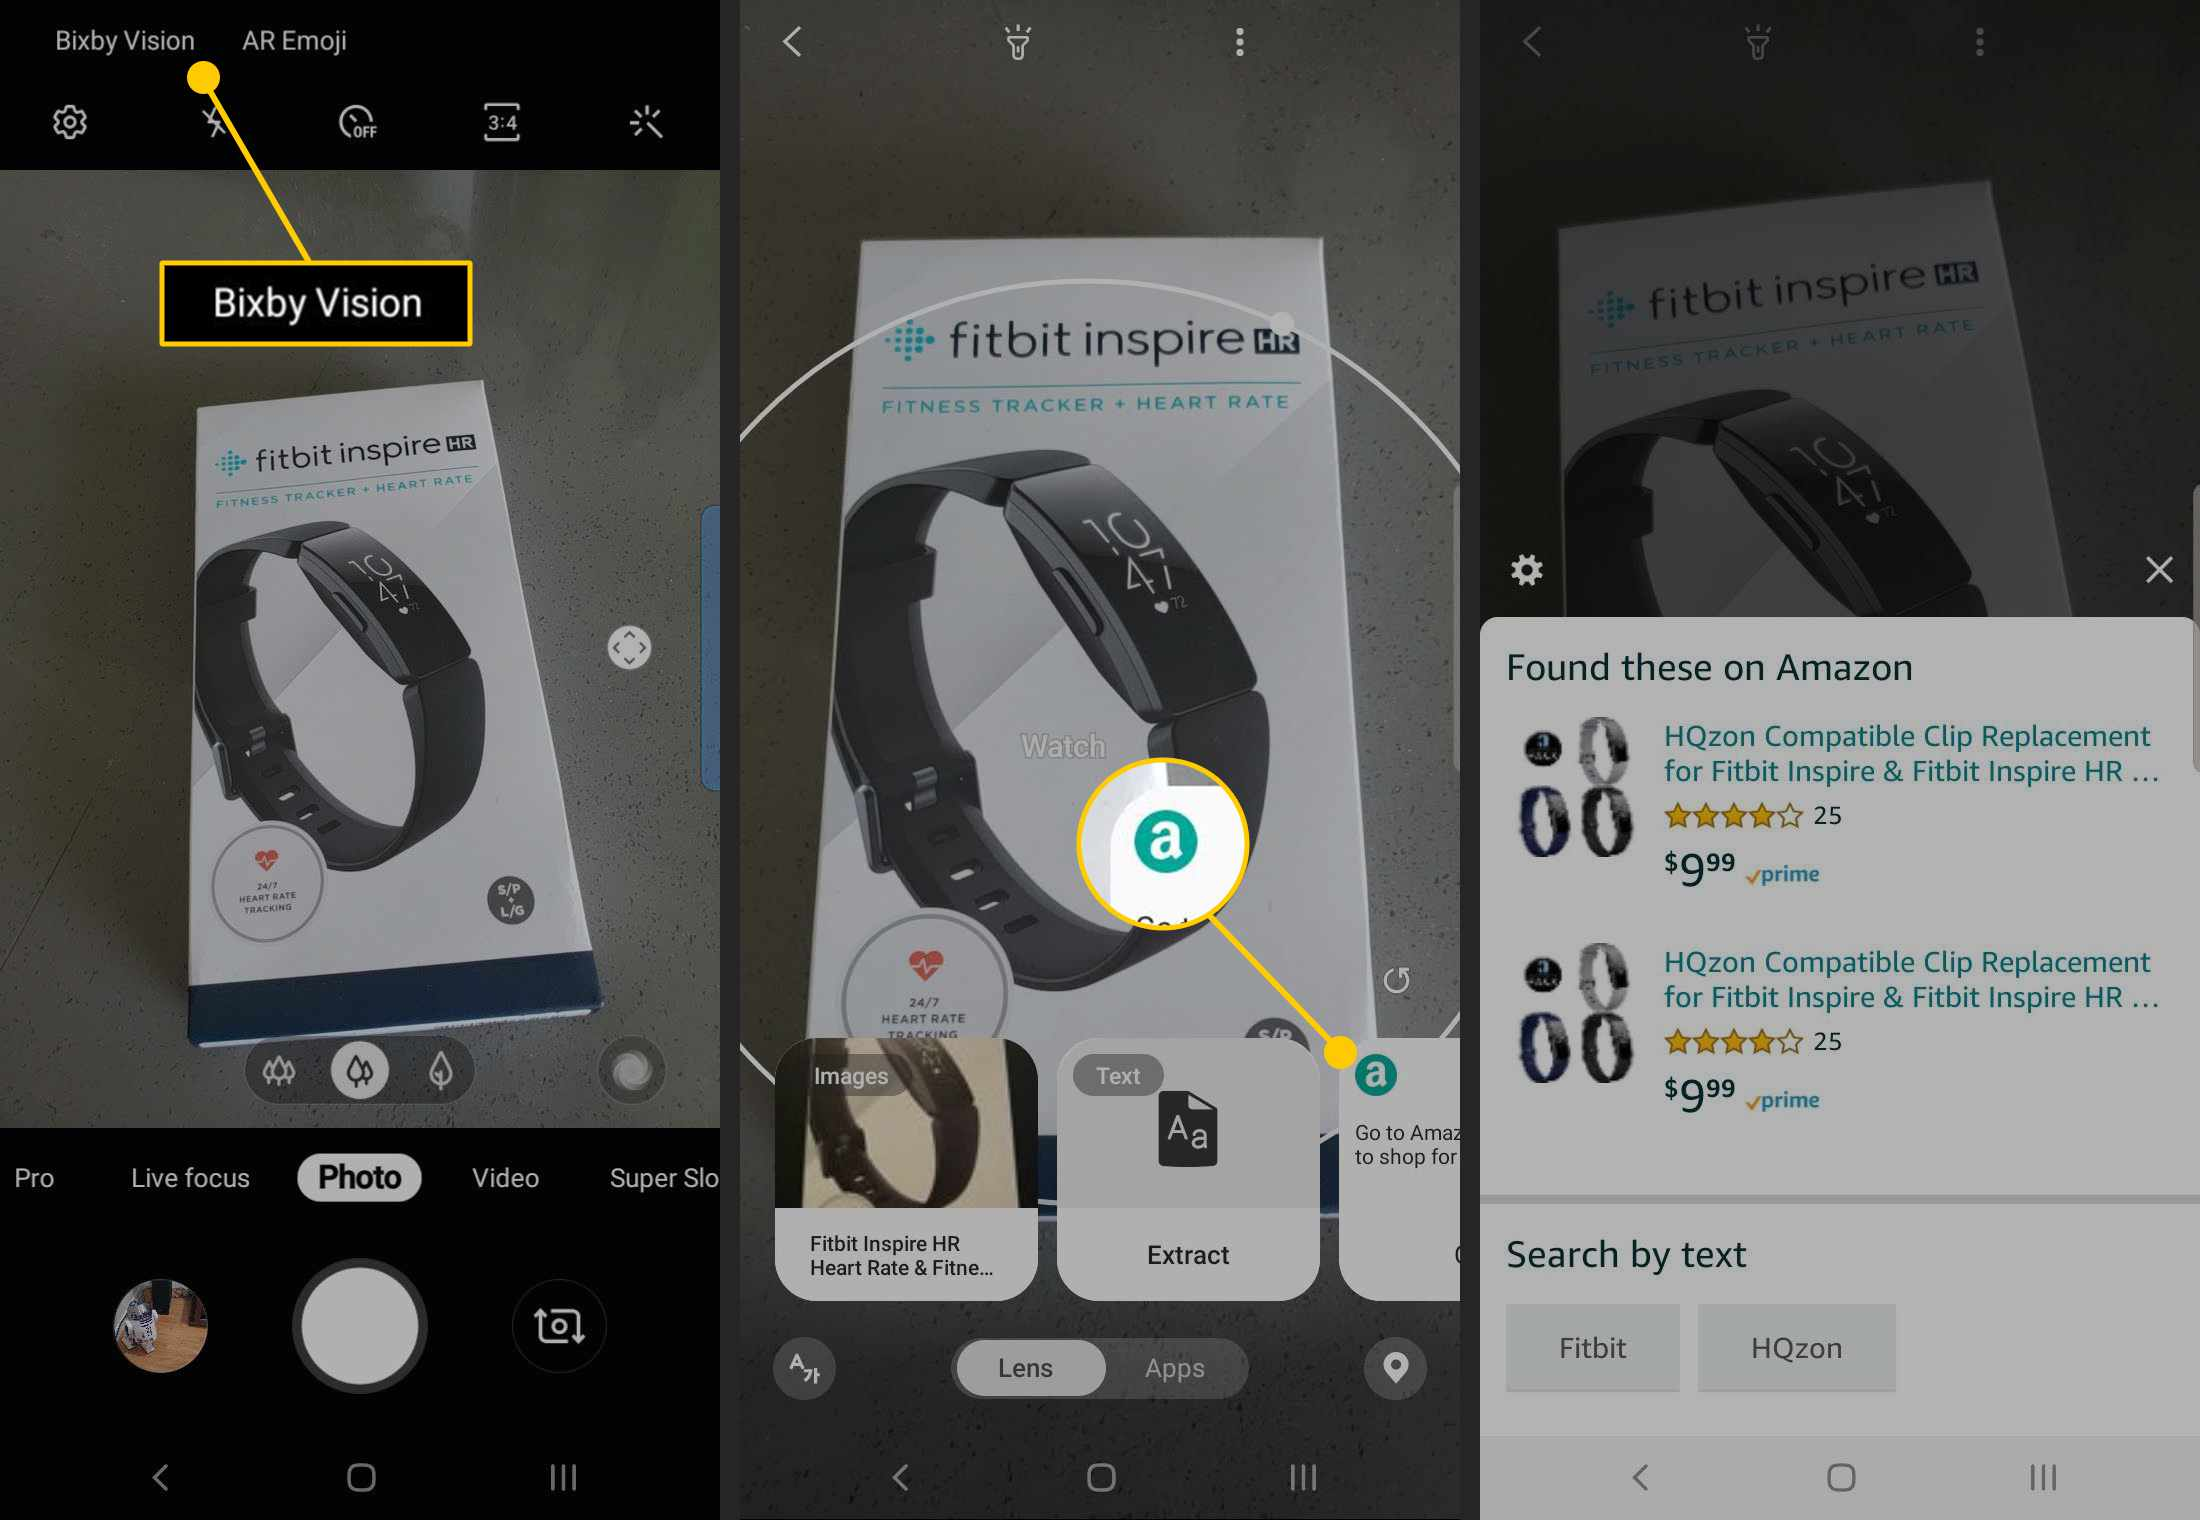
\includegraphics[width=0.5\linewidth]{bixby3.jpg}
	\caption{Bixby Vision, Reconocimiento de imagenes.}
	\label{fig:Irecog2}
\end{figure}

\subsubsection{Google Lens}
Google lens es una aplicación móvil de reconocimiento de imagen diseñada para mostrar información, a partir del análisis de una imagen, generando varios resultados posibles y clasificarlos según la relevancia. Por ejemplo, si una imagen incluye un producto específico (ropas o jeans), puede mostrar resultados que brinden más información sobre el producto o que ofrezcan opciones para comprarlo. Puede utilizar códigos de barras o texto en una imagen, con esto puede mostrar una página de resultados. Tiene varias funciones: comprender lo que se está mirando, traducir texto o copiar, identificar algún animal o objeto, explorar lugares o menús, descubrir productos, entre otros.\cite{lens.google2021}
\begin{figure} 	
	%\centering
	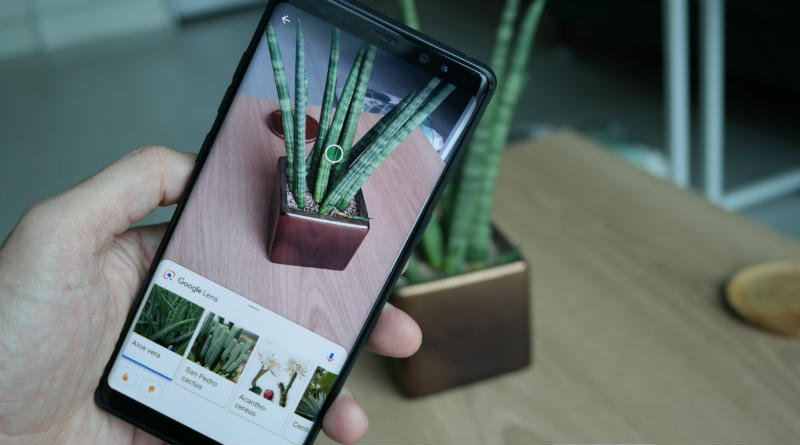
\includegraphics[width=0.5\linewidth]{Google-Lens-1.jpg}
	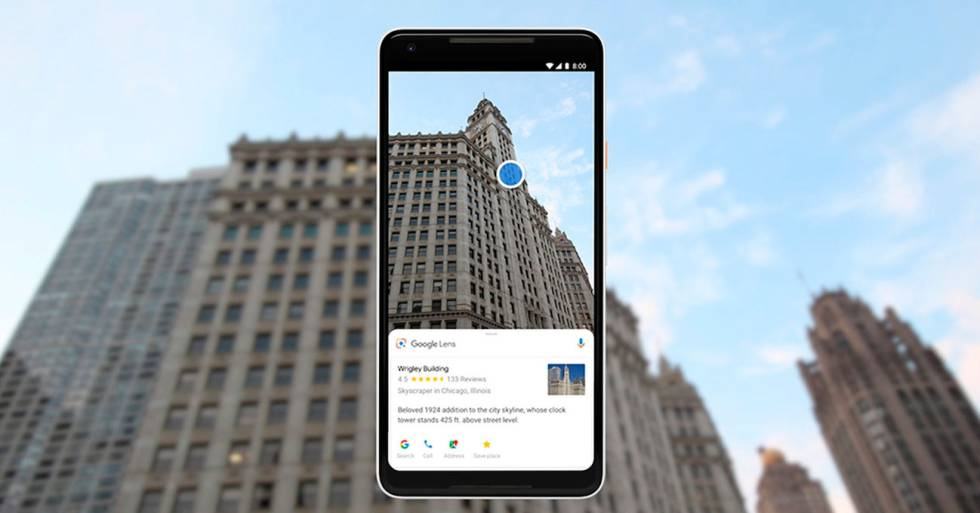
\includegraphics[width=0.5\linewidth]{Google-Lens-2.jpg}
	\caption{Google Lens, Reconocimiento de imagenes.}
	\label{fig:Irecog3}
\end{figure}


\subsection{LinkRay Light ID}

LinkRay es una tecnología de que permite transmitir información a un teléfono móvil que cuenta con la aplicación, a través de la luz led visible, por medio de los letreros LED y pantallas LED, entre otros. También son usadas en la comunicación, en el marketing, industrias de turismo, venta minorista, hotelería, transporte y gestión de eventos. Por ejemplo, informar las condiciones del tráfico en tiempo real, ofrecer cupones en comercios, publicidad dirigida a usuarios optativos como forma de aumento de las ventas y el servicio.
A partir de la luz que emiten los transmisores LED, es posible leer las etiquetas identificativas. Los datos enviados al usuario pueden ser archivos de imagen, audio o vídeo. \cite{Business2017}
\\
\textbf{Ventajas}: Velocidad de transmisión por medio de la luz led visible.\cite{Business2017}
\\
\textbf{Desventajas}: En desarrollo desde su presentación en 2017\cite{Business2017}

\begin{figure} 	
	%\centering
	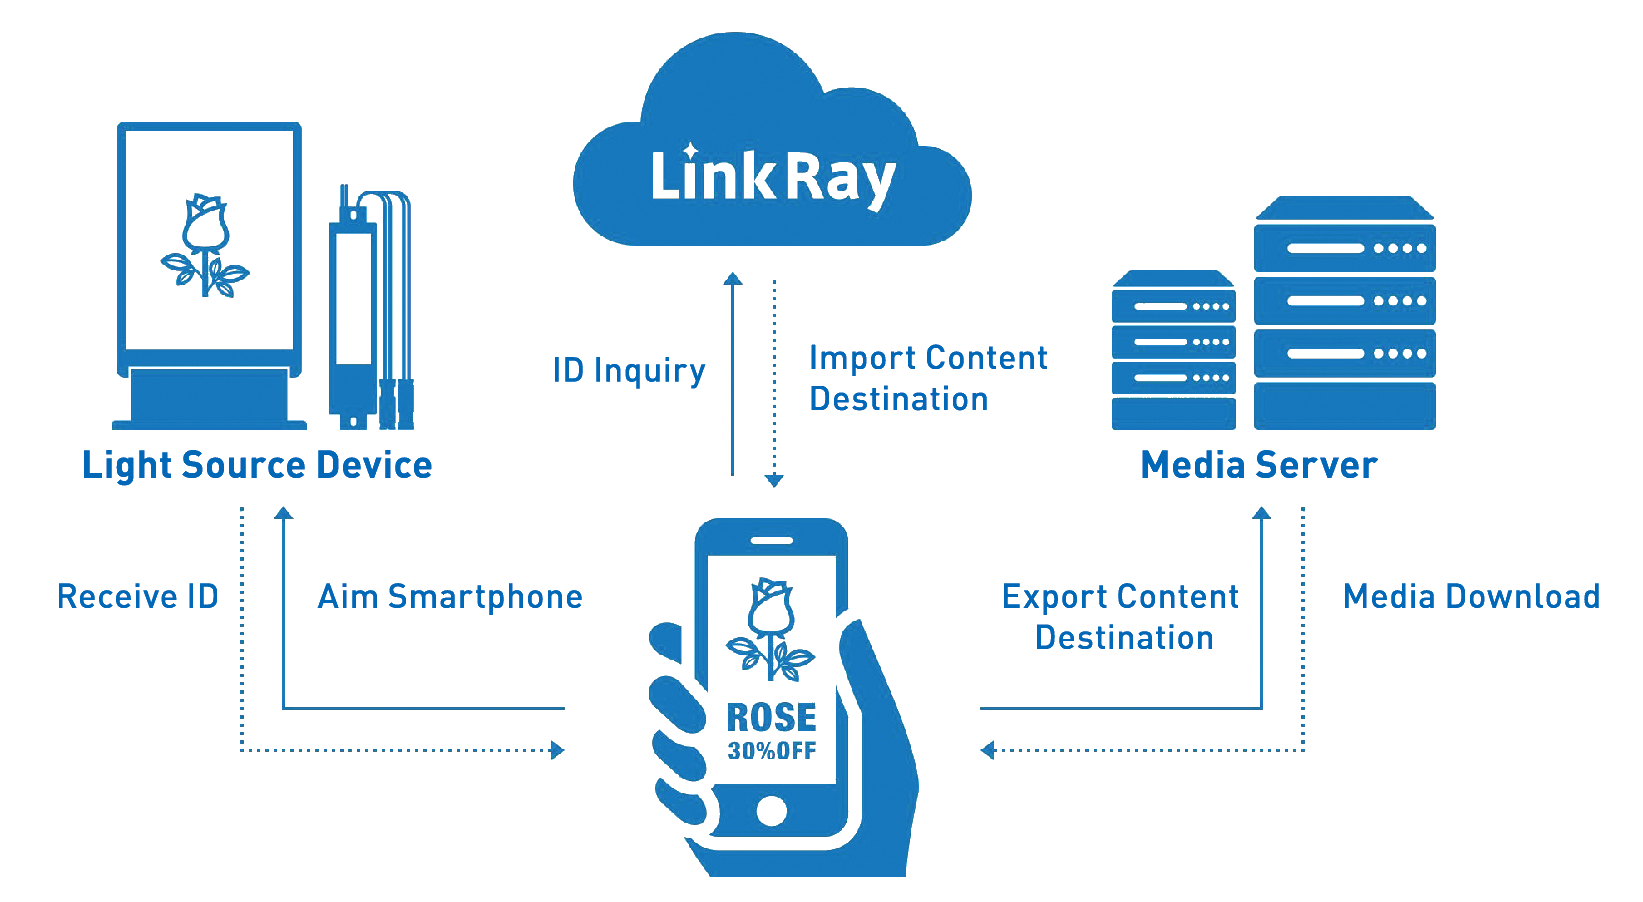
\includegraphics[width=0.5\linewidth]{linkray_system_configuration_1.png}
	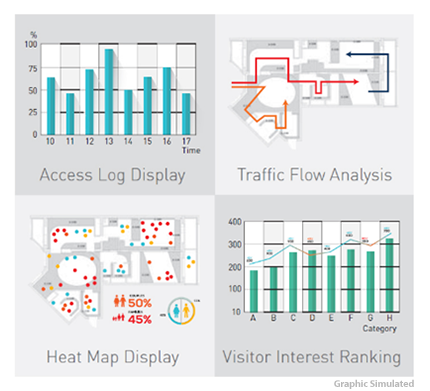
\includegraphics[width=0.4\linewidth]{LinKRayGraphs.png}
	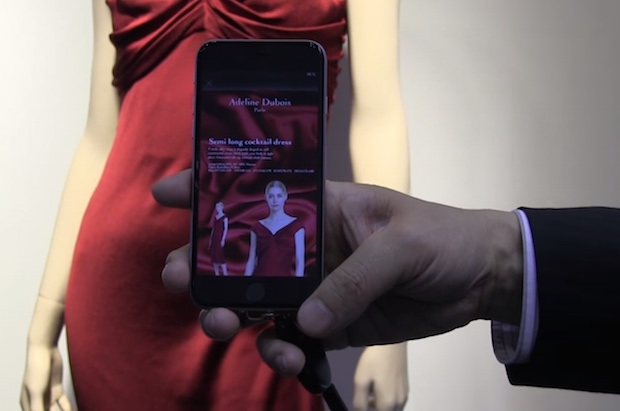
\includegraphics[width=0.4\linewidth]{Panasonic-Light-ID.jpg}
	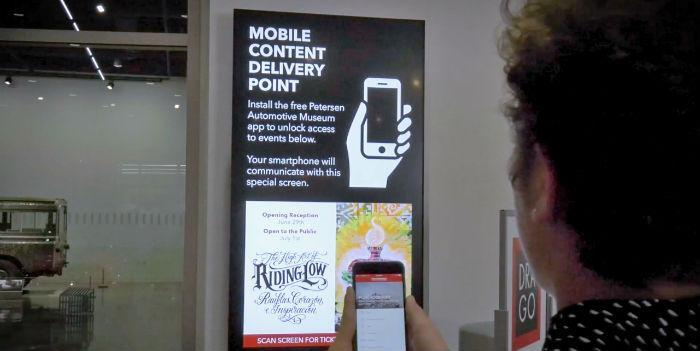
\includegraphics[width=0.5\linewidth]{linkrayMuseum.jpg}
	\caption{Tecnología LinkRay Light ID.}
	\label{fig:linkray}
\end{figure}


